\subsection{Benchmark problems}
% USE gp grid parameters
% Experiments
% shared experiments
Recent work on the convergence of GP-based SR \cite{SRAccur, SRBaseline} featured a set of benchmark problems that pose convergence problems for SR implementations. We reuse these problems in our work in order to study convergence of CSRM's implementation.
\subsubsection{Problems}
These problems use at most five features. CSRM does not know which features are used, making the problem harder. In other words it assumes each problem is a function of 5 features which may or may not influence the expected outcome. This is an extra test in robustness for the algorithm, while also testing the algorithm's capability as a classifier. These problems are introduced by \cite{SRBaseline}.
\[
1.57 + (24.3*x_3)\]
\[0.23+14.2*\frac{x_3+x_1}{3.0*x_4}
\]
\[
-5.41 + 4.9* ( \frac{x_3-x_0 +  \frac{x_1}{x_4} } {3*x_4} )
\] 
\[-2.3 + 0.13*\sin(x_2)\]
\[3.0 + (2.13 * ln(x_4))\]
\[1.3 + 0.13* \sqrt{x_0}\]
\[213.80940889 - 213.80940889*e^{-0.54723748542*x_0}\]
\[6.87+11*\sqrt{7.23*x_0*x_3*x_4}\]
\[\frac{\sqrt{x_0}}{\ln(x_1)} *\frac{e^{x_2}}{x_3 ^ 2}\]
\[ 0.81 + 24.3 * \frac{ 2.0*x_1+3.0*x_2^2} {4.0*x_3^3 + 5.0*x_4^4}\]
\[6.87+ 11* \cos(7.23*x_0^3)\]
\[2.0 - 2.1 * \cos(9.8*x_0) * \sin(1.3*x_4)\]
\[32-3.0*  \frac{\tan(x_0)}{\tan(x_1)} *  \frac{tan(x_2)} {\tan(x_3)} \]
\[22 - 4.2*((\cos(x_0)-\tan(x_1))*\frac{\tanh(x_2)}{\sin(x_3)}\]
\[12.0 - 6.0* \frac{\tan(x_0)}{e^{x_1}} * (\ln(x_2)-\tan(x_3) ) \]
                    

\subsection{Operators}
../hybrid/sharedexperiments.tex
% Show the effect of cooling
% Show the effect of depth sensitive

% Exclusive experiments
\subsection{Constant Folding}\ref{subsecctfold}
\subsubsection{Savings}
% Show effect of constant folding savings
% Explain how, even thoug small, these savings add up, e.g. 1% bloat increases.

\subsection{Constant optimization}
We look at the effect constant optimization using different algorithms has on different configurations of the tool. The measures used in the comparison are best fitness on training and test data, mean fitness on training and test data, and optimization cost.

\subsubsection{Test problem}
To verify our implementation for the optimizers we use a simple test problem and observe for each optimizer if it is able to optimize this instance to a known optimal value.
\[
f(x_0, x_1, x_2) = 1 + x_1 * \sin (5+x_2) * x_0 + (17 + \sin (233+9))
\]
We give each optimizer a population of 50, 50 iterations and compare the results for 10 runs, displaying best value obtained, mean, and standard deviation of the fitness values compared to the known best value.
\paragraph{Best fitness}
In Figure \ref{fig:testproblembest} we see that DE outperforms PSO and ABC with several orders of magnitude. The best fitness value obtained was 2.22 e-16. As smaller but significant difference is present between PSO and ABC. This result is somewhat surprising given that fact that ABC is allowed to perform more evaluations in its configuration. From our previous discussion \ref{psocost},\ref{decost},\ref{abccost} we can conclude that for this test problem DE is clearly preferable as it obtains the best result at minimum cost. ABC has almost double the cost compared to PSO and DE, with PSO and DE having an equal cost in evaluations. The results on this testproblem do not necessarily mean that in the application of the three optimizers the results will be identical. Here we have a known optimal solution and want to observe how fast the optimizers converge to it. When we optimize evolved expressions we do not know what the optimal solution is. The problem statement is different, and so the convergence behavior is likely to differ as well. 
\paragraph{Distribution of fitness}
In Figures \ref{fig:testproblemmean} and \ref{fig:testproblemsd} we see that both the mean and standard deviation follow the same pattern as seen for the minimum fitness value with DE leading the others by several orders of magnitude. With all three distributions behaving similarly, this result provides a more solid foundation for our conclusions that for this problem DE is indeed the better optimizer.
\begin{figure}
    \centering
    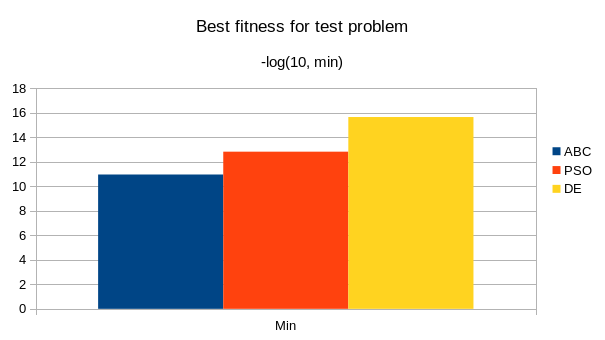
\includegraphics[width=\textwidth,height=\textheight,keepaspectratio]{figures/testproblem_bestfitness.png}
    \caption{Logarithmic value of best fitness for each optimizer.}
    \label{fig:testproblembest}
\end{figure}
\begin{figure}
    \centering
    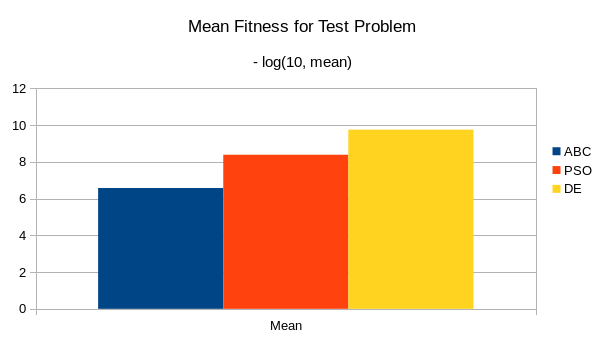
\includegraphics[width=\textwidth,height=\textheight,keepaspectratio]{figures/testproblem_meanfitness.png}
    \caption{Logarithmic scaled mean fitness for each optimizer.}
    \label{fig:testproblemmean}
\end{figure}
\begin{figure}
    \centering
    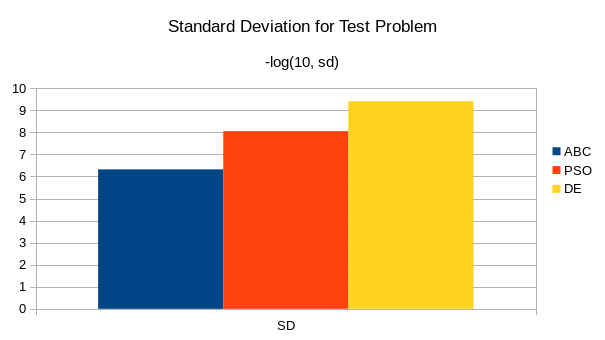
\includegraphics[width=\textwidth,height=\textheight,keepaspectratio]{figures/testproblem_sdfitness.png}
    \caption{Logarithmic scaled standard deviation fitness for each optimizer.}
    \label{fig:testproblemsd}
\end{figure}

\subsubsection{Optimizer experiments setup}
We test the 15 expressions with the following configuration:
\begin{itemize}
\item population : 20
\item minimum depth : 4
\item maximum depth : 10
\item phases : (2, 5, 10)
\item generations per phase : 20
\item datapoints : 20
\item range : [1,5]
\item features : 5
\item archivesize : 20
\item expressions to archive per phase : 4
\item optimization strategy : optimize expressions archived at end of phase
\end{itemize}
\subsubsection{Measures}
We compare the relative gain in fitness compared to not using an optimizer for all expressions. 
In other words, if $m_n$ is a measure obtained by the algorithm without the optimizer, and $m_a$ the same measure with the optimizer, we then define the relative gain as :
\[
g_{ma} = \frac{m_n}{m_a}
\]
If $m_a$ is zero, we use $-log_{10}(m_n)$ to represent the gain. If both are zero, the gain is obviously 1. A value of g $>$ 1 indicates the ratio with which the optimizer improves the result. A g value $<$ 1 indicates a regression.
These 15 functions have wildly varying convergence behavior. In order to make sense of the data, we then apply a log scale :
\[
g_{lma} = - \log_{10}(g_{ma})
\]
A value of $g_{lma} > 0 $ indicates improvement, with the units transformed to orders of magnitude. A zero value indicates no improvement is registered, and negative values indicate regression. 
As measures we use the best fitness value on the training data, and the best on the full data set. We take the mean of the fitness of the 5 best expressions on training and the full data as well. This last measure gives us an indication on how the optimization process acts on the 'best' set of the population. Note that in our configuration, the 4 best expressions are always optimized.
\subsubsection{2 Phases}
In Figure \ref{fig:2phase} we see the performance of the algorithms on training data. 
In Table \ref{table:2phasemintrain} we see that for problems 0, 4, 5 there is no improvement possible (e.g. 0 zero fitness value), which explains the absence of any value in the figure.
We see that for the training fitness data the improvements are significant, with ABC scoring an increase of 2.5 orders of magnitude for problem 6. For the other problems the increase is still large, especially given that our fitness function has a range of [0,1].
We also observe the significant regression for problem 6. This is likely caused due to overfitting. The algorithm in question (DE) optimizes the 4 best candidates of the last phase (1), but it is possible that these optimized expressions actually form a local optimum. By archiving these the convergence of the algorithm is hindered in the next phase. Note that DE allows equality updates, where expressions with the same fitness values are accepted as better. The same behavior occurs in a far less significant effect for expressions 7 and 9. A second explanation is our implementation of the population. The algorithm enforces distinct fitness values for all expressions. In an edge case it is possible that these optimized samples form a barrier, preventing other expressions from evolving past them. The optimized expressions in effect trap the rest of the population, which given our low generation count can explain this behavior.
The mean fitness of the 5 best expressions shows significant improvements. Important to observe is the similarity between the two plots, the correlation between fitness values on training and full data is strong. This was a concern in the setup of the experiments. The optimizers could introduce overfitting on the training data. This risk is mitigated by the relatively low number of iterations each optimizer has been allocated.
For the minimum fitness on the full data ABC outperforms the others. For the mean evaluation PSO is a good candidate. In this stage of the experiments, there is no single algorithm that is ideal for all problems. This once again confirms the NFL theorem \cite{NFL}.

% Figures
\begin{figure}
    \centering
    \begin{subfigure}{0.6\textwidth}
    \centering
        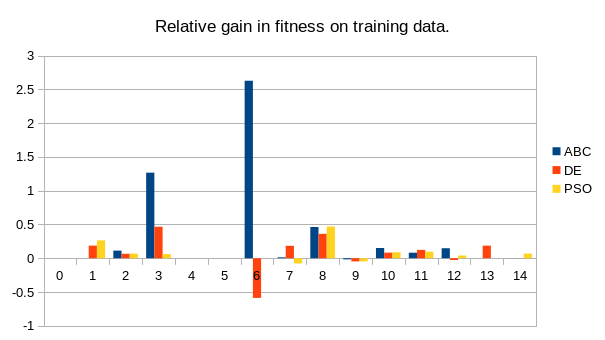
\includegraphics[width=0.8\linewidth]{figures/hybrid_phases2_mintrainfitness.png}
        \caption{Relative gain in best fitness of training data}
    \end{subfigure}%
    \begin{subfigure}{0.6\textwidth}
    \centering
        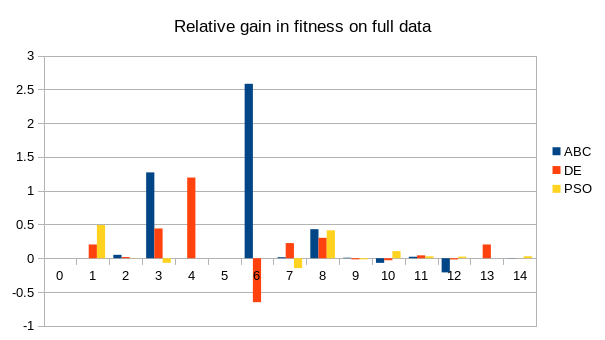
\includegraphics[width=0.8\linewidth]{figures/hybrid_phases2_minfullfitness.png}
        \caption{Relative gain in best fitness of full data}
    \end{subfigure}
        \begin{subfigure}{0.6\textwidth}
    \centering
        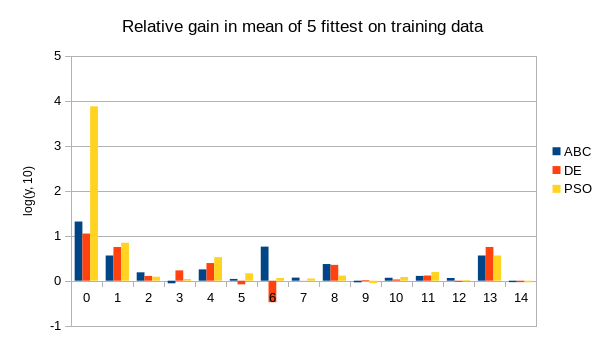
\includegraphics[width=0.8\linewidth]{figures/hybrid_phases2_meantrainfitness.png}
        \caption{Relative gain in mean fitness of training data}
    \end{subfigure}%
    \begin{subfigure}{0.6\textwidth}
    \centering
        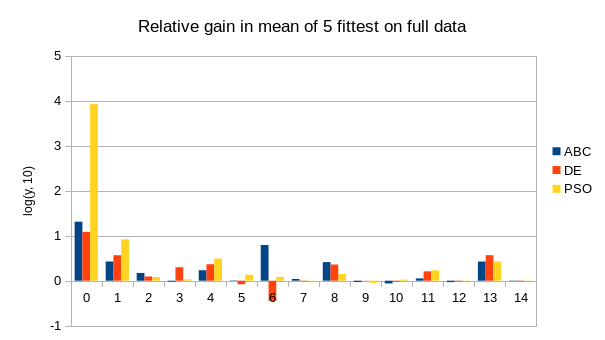
\includegraphics[width=0.8\linewidth]{figures/hybrid_phases2_meanfullfitness.png}
        \caption{Relative gain in mean fitness of full data}
    \end{subfigure}
    \caption{Relative gain of optimizer after 2 phases.}
    \label{fig:2phase}
    \end{figure}

% Table
\begin{landscape}
\begin{table}[]
\centering
\caption{Relative Gain in minimum fitness on training data after 2 phases.}
\label{table:2phasemintrain}
\begin{adjustbox}{width=1.7\textwidth}
\begin{tabular}{lllllllllllllllll}
          &           &           &           &           &           &           &           &           &           &           &           &           &           &           &           &  \\
           & 0         & 1         & 2         & 3         & 4         & 5         & 6         & 7         & 8         & 9         & 10        & 11        & 12        & 13        & 14        &  \\
ABC                 & 1.000e+00 & 1.000e+00 & 1.295e+00 & 1.848e+01 & 1.000e+00 & 1.000e+00 & 4.253e+02 & 1.030e+00 & 2.897e+00 & 9.615e-01 & 1.415e+00 & 1.207e+00 & 1.404e+00 & 1.000e+00 & 9.970e-01 &  \\
DE                  & 1.000e+00 & 1.536e+00 & 1.163e+00 & 2.923e+00 & 1.000e+00 & 1.000e+00 & 2.584e-01 & 1.526e+00 & 2.294e+00 & 8.972e-01 & 1.210e+00 & 1.327e+00 & 9.397e-01 & 1.536e+00 & 9.960e-01 &  \\
PSO                 & 1.000e+00 & 1.839e+00 & 1.169e+00 & 1.150e+00 & 1.000e+00 & 1.000e+00 & 1.000e+00 & 8.356e-01 & 2.947e+00 & 8.971e-01 & 1.226e+00 & 1.247e+00 & 1.096e+00 & 1.000e+00 & 1.172e+00 &  \\

\end{tabular}
\end{adjustbox}
\end{table}

\begin{table}[]
\centering
\caption{Gain in minimum fitness on full data after 2 phases.}
\label{table:2phaseminfull}
\begin{adjustbox}{width=1.7\textwidth}
\begin{tabular}{lllllllllllllllll}
         &           &           &           &           &           &           &           &           &           &           &           &           &           &           &           &  \\
         & 0         & 1         & 2         & 3         & 4         & 5         & 6         & 7         & 8         & 9         & 10        & 11        & 12        & 13        & 14        &  \\
ABC                 & 1.000e+00 & 1.000e+00 & 1.122e+00 & 1.865e+01 & 1.000e+00 & 1.000e+00 & 3.831e+02 & 1.034e+00 & 2.691e+00 & 1.016e+00 & 8.528e-01 & 1.051e+00 & 6.169e-01 & 1.000e+00 & 9.938e-01 &  \\
DE                  & 1.000e+00 & 1.597e+00 & 1.039e+00 & 2.757e+00 & 1.565e+01 & 1.000e+00 & 2.233e-01 & 1.674e+00 & 2.004e+00 & 9.617e-01 & 9.337e-01 & 1.103e+00 & 9.584e-01 & 1.597e+00 & 9.970e-01 &  \\
PSO                 & 1.000e+00 & 3.098e+00 & 9.915e-01 & 8.538e-01 & 1.000e+00 & 1.000e+00 & 1.000e+00 & 7.145e-01 & 2.586e+00 & 9.617e-01 & 1.274e+00 & 1.067e+00 & 1.055e+00 & 1.000e+00 & 1.069e+00 &  \\
\end{tabular}
\end{adjustbox}
\end{table}

\begin{table}[]
\centering
\caption{Relative gain in mean fitness of 5 fittest expressions on training data after 2 phases.}
\label{table:2phasemeantrain}
\begin{adjustbox}{width=1.7\textwidth}
\begin{tabular}{lllllllllllllllll}
&           &           &           &           &           &           &           &           &           &           &           &           &           &           &           &  \\
           & 0         & 1         & 2         & 3         & 4         & 5         & 6         & 7         & 8         & 9         & 10        & 11        & 12        & 13        & 14        &  \\
ABC                 & 1.335e+01 & 1.113e+00 & 4.824e+00 & 5.543e-01 & 3.479e+02 & 4.395e+02 & 7.059e-02 & 4.477e-01 & 1.215e+00 & 9.073e-01 & 2.214e+00 & 9.169e-01 & 1.564e+00 & 1.113e+00 & 4.064e-01 &  \\
DE                  & 3.620e+01 & 1.299e+00 & 1.115e+00 & 1.128e+00 & 1.204e-01 & 5.385e+08 & 3.202e+01 & 1.338e+00 & 1.835e+00 & 1.154e+00 & 1.268e+00 & 1.626e+00 & 1.246e+00 & 1.299e+00 & 7.247e-01 &  \\
PSO                 & 5.046e+02 & 8.017e+00 & 2.302e+00 & 4.220e-01 & 1.665e+01 & 2.237e+01 & 2.144e-01 & 6.974e-01 & 1.240e+00 & 9.647e-01 & 1.408e+00 & 1.347e+00 & 5.933e+00 & 7.152e-01 & 8.523e-01 &  \\


\end{tabular}
\end{adjustbox}
\end{table}


\begin{table}[]
\centering
\caption{Relative gain in mean fitness of 5 fittest expressions on full data after 2 phases.}
\label{table:2phasemeanfull}
\begin{adjustbox}{width=1.7\textwidth}
\begin{tabular}{lllllllllllllllll}
 meanfullfitness     &           &           &           &           &           &           &           &           &           &           &           &           &           &           &           &  \\
algorithm           & 0         & 1         & 2         & 3         & 4         & 5         & 6         & 7         & 8         & 9         & 10        & 11        & 12        & 13        & 14        &  \\
ABC                 & 1.382e+01 & 2.306e-01 & 5.950e+00 & 5.551e-01 & 3.264e+02 & 5.091e+02 & 7.308e-02 & 4.463e-01 & 1.188e+00 & 9.214e-01 & 4.665e-01 & 7.197e-01 & 1.463e+00 & 2.306e-01 & 8.096e-01 &  \\
DE                  & 3.244e+01 & 1.315e+00 & 1.068e+00 & 1.228e+00 & 1.153e-01 & 5.392e+08 & 3.234e+01 & 1.348e+00 & 1.685e+00 & 1.153e+00 & 1.193e+00 & 1.441e+00 & 1.210e+00 & 1.315e+00 & 1.199e+00 &  \\
PSO                 & 4.920e+02 & 6.794e+00 & 2.531e+00 & 4.117e-01 & 1.721e+01 & 9.994e+00 & 2.146e-01 & 6.486e-01 & 1.113e+00 & 7.060e-01 & 5.830e-01 & 1.324e+00 & 2.613e+00 & 8.126e-01 & 1.094e+00 & \\

\end{tabular}
\end{adjustbox}
\end{table}
\end{landscape}



\subsubsection{5 Phases}
With 5 phases we see in Figure\ref{fig:5phase} a more diverse effect. While ABC scores exceptionally good on problem 6, in sharp contrast with the 2 phase experiment, we see that PSO scores overall better for the training data. These results are logarithmic scaled, an improvement in fitness of factor 10 results in a value of 1 in the plots. When it comes to improving the mean of the best 5 expressions, PSO is a stable choice if we disregard the outlier values for problem 5. The correlation between training and full fitness scores is good for both measures. This demonstrates that the optimizer is not in this experiment introducing overfitting on the training data. The adverse effect of the optimizer on some test problems is still present.
For the best fitness values on the full data DE is the better candidate. While ABC scores exceptionally high on problem 6, DE scores better overall. When we look at the mean there is no clear winner. 
\begin{figure}
    \centering
    \begin{subfigure}{0.6\textwidth}
    \centering
        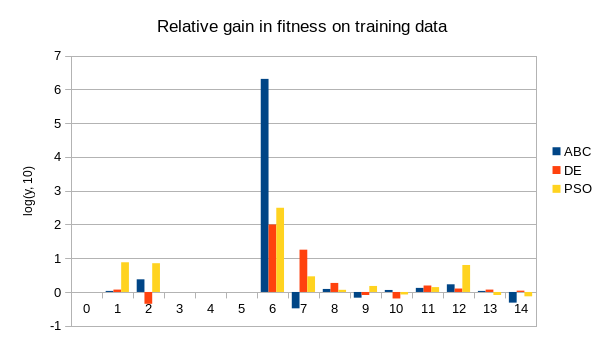
\includegraphics[width=0.8\linewidth]{figures/hybrid_phases5_mintrainfitness.png}
        \caption{Relative gain in best fitness of training data}
    \end{subfigure}%
    \begin{subfigure}{0.6\textwidth}
    \centering
        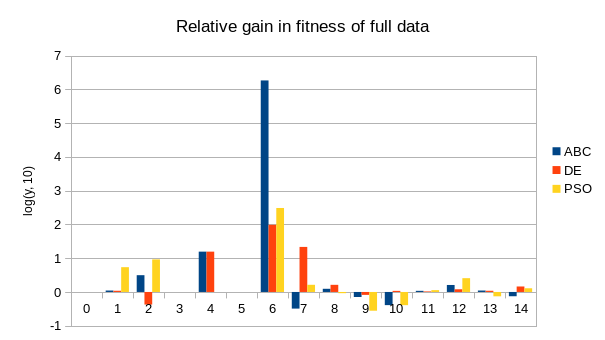
\includegraphics[width=0.8\linewidth]{figures/hybrid_phases5_minfullfitness.png}
        \caption{Relative gain in best fitness of full data}
    \end{subfigure}
        \begin{subfigure}{0.6\textwidth}
    \centering
        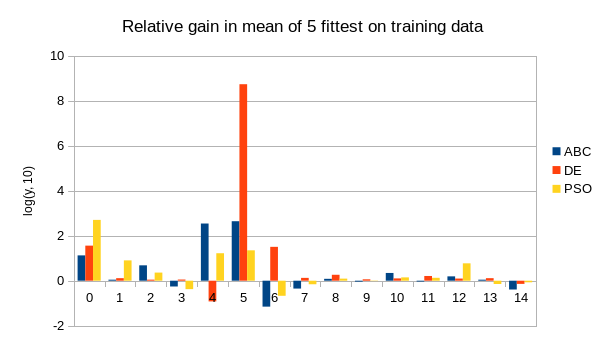
\includegraphics[width=0.8\linewidth]{figures/hybrid_phases5_meantrainfitness.png}
        \caption{Relative gain in mean fitness of training data}
    \end{subfigure}%
    \begin{subfigure}{0.6\textwidth}
    \centering
        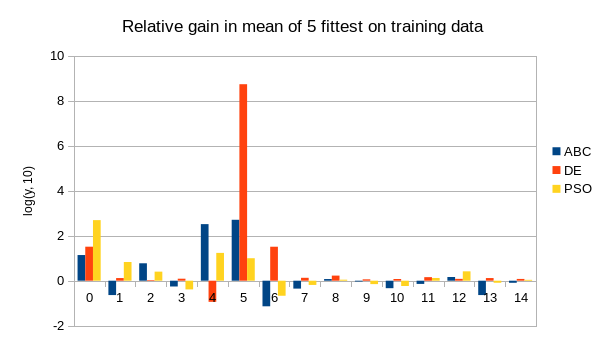
\includegraphics[width=0.8\linewidth]{figures/hybrid_phases5_meanfullfitness.png}
        \caption{Relative gain in mean fitness of full data}
    \end{subfigure}
    \caption{Relative gain of optimizer after 5 phases.}
    \label{fig:5phase}
    \end{figure}

% Table
\begin{landscape}
\begin{table}[]
\centering
\caption{Relative Gain in minimum fitness on training data after 5 phases.}
\label{table:5phasemintrain}
\begin{adjustbox}{width=1.7\textwidth}
\begin{tabular}{lllllllllllllllll}
     &           &           &           &           &           &           &           &           &           &           &           &           &           &           &           &  \\
algorithm           & 0         & 1         & 2         & 3         & 4         & 5         & 6         & 7         & 8         & 9         & 10        & 11        & 12        & 13        & 14        &  \\
ABC                 & 1.000e+00 & 1.074e+00 & 2.371e+00 & 1.000e+00 & 1.000e+00 & 1.000e+00 & 2.050e+06 & 3.277e-01 & 1.230e+00 & 6.779e-01 & 1.146e+00 & 1.321e+00 & 1.690e+00 & 1.074e+00 & 4.837e-01 &  \\
DE                  & 1.000e+00 & 1.176e+00 & 4.459e-01 & 1.000e+00 & 1.000e+00 & 1.000e+00 & 9.987e+01 & 1.790e+01 & 1.853e+00 & 8.129e-01 & 6.428e-01 & 1.553e+00 & 1.266e+00 & 1.176e+00 & 1.095e+00 &  \\
PSO                 & 1.000e+00 & 7.591e+00 & 7.112e+00 & 0.000e+00 & 1.000e+00 & 1.000e+00 & 3.117e+02 & 2.904e+00 & 1.159e+00 & 1.506e+00 & 8.442e-01 & 1.396e+00 & 6.302e+00 & 8.146e-01 & 7.435e-01 &  \\

\end{tabular}
\end{adjustbox}
\end{table}

\begin{table}[]
\centering
\caption{Gain in minimum fitness on full data after 5 phases.}
\label{table:5phaseminfull}
\begin{adjustbox}{width=1.7\textwidth}
\begin{tabular}{lllllllllllllllll}
            &           &           &           &           &           &           &           &           &           &           &           &           &           &           &           &  \\
           & 0         & 1         & 2         & 3         & 4         & 5         & 6         & 7         & 8         & 9         & 10        & 11        & 12        & 13        & 14        &  \\
ABC                 & 1.000e+00 & 1.103e+00 & 3.145e+00 & 1.000e+00 & 1.565e+01 & 1.000e+00 & 1.846e+06 & 3.220e-01 & 1.243e+00 & 7.106e-01 & 4.082e-01 & 1.080e+00 & 1.613e+00 & 1.103e+00 & 7.483e-01 &  \\
DE                  & 1.000e+00 & 1.087e+00 & 4.240e-01 & 1.000e+00 & 1.565e+01 & 1.000e+00 & 9.756e+01 & 2.158e+01 & 1.629e+00 & 8.213e-01 & 1.079e+00 & 1.040e+00 & 1.202e+00 & 1.087e+00 & 1.454e+00 &  \\
PSO                 & 1.000e+00 & 5.426e+00 & 9.234e+00 & 0.000e+00 & 1.000e+00 & 1.000e+00 & 3.070e+02 & 1.634e+00 & 9.216e-01 & 2.786e-01 & 4.071e-01 & 1.131e+00 & 2.563e+00 & 7.444e-01 & 1.288e+00 &  \\

\end{tabular}
\end{adjustbox}
\end{table}

\begin{table}[]
\centering
\caption{Relative gain in mean fitness of 5 fittest expressions on training data after 5 phases.}
\label{table:5phasemeantrain}
\begin{adjustbox}{width=1.7\textwidth}
\begin{tabular}{lllllllllllllllll}
 &           &           &           &           &           &           &           &           &           &           &           &           &           &           &           &  \\
           & 0         & 1         & 2         & 3         & 4         & 5         & 6         & 7         & 8         & 9         & 10        & 11        & 12        & 13        & 14        &  \\
ABC                 & 2.064e+01 & 3.632e+00 & 1.536e+00 & 8.774e-01 & 1.788e+00 & 1.096e+00 & 5.726e+00 & 1.173e+00 & 2.348e+00 & 9.209e-01 & 1.163e+00 & 1.280e+00 & 1.151e+00 & 3.632e+00 & 9.300e-01 &  \\
DE                  & 1.117e+01 & 5.624e+00 & 1.277e+00 & 1.696e+00 & 2.468e+00 & 8.307e-01 & 3.333e-01 & 9.953e-01 & 2.249e+00 & 1.038e+00 & 1.067e+00 & 1.305e+00 & 9.416e-01 & 5.624e+00 & 9.302e-01 &  \\
PSO                 & 7.494e+03 & 6.977e+00 & 1.225e+00 & 1.091e+00 & 3.335e+00 & 1.461e+00 & 1.154e+00 & 1.118e+00 & 1.300e+00 & 8.794e-01 & 1.212e+00 & 1.559e+00 & 1.041e+00 & 3.632e+00 & 9.242e-01 &  \\

\end{tabular}
\end{adjustbox}
\end{table}


\begin{table}[]
\centering
\caption{Relative gain in mean fitness of 5 fittest expressions on full data after 5 phases.}
\label{table:5phasemeanfull}
\begin{adjustbox}{width=1.7\textwidth}
\begin{tabular}{lllllllllllllllll}
    &           &           &           &           &           &           &           &           &           &           &           &           &           &           &           &  \\
    & 0         & 1         & 2         & 3         & 4         & 5         & 6         & 7         & 8         & 9         & 10        & 11        & 12        & 13        & 14        &  \\
ABC                 & 2.048e+01 & 2.672e+00 & 1.487e+00 & 9.516e-01 & 1.709e+00 & 1.021e+00 & 6.217e+00 & 1.093e+00 & 2.589e+00 & 9.346e-01 & 8.686e-01 & 1.126e+00 & 9.308e-01 & 2.672e+00 & 9.816e-01 &  \\
DE                  & 1.213e+01 & 3.687e+00 & 1.244e+00 & 1.997e+00 & 2.324e+00 & 8.352e-01 & 3.572e-01 & 9.731e-01 & 2.288e+00 & 1.009e+00 & 9.496e-01 & 1.616e+00 & 9.641e-01 & 3.687e+00 & 9.668e-01 &  \\
PSO                 & 8.382e+03 & 8.286e+00 & 1.204e+00 & 1.071e+00 & 3.111e+00 & 1.362e+00 & 1.219e+00 & 9.817e-01 & 1.411e+00 & 8.939e-01 & 1.059e+00 & 1.698e+00 & 1.018e+00 & 2.672e+00 & 9.840e-01 & 

\end{tabular}
\end{adjustbox}
\end{table}
\end{landscape}

\subsubsection{10 Phases}
If we observe the convergence after 10 phases we see a more pronounced effect. In Figure \ref{fig:10phase} we see that for several problems the optimizers are no longer improving w.r.t the unoptimized algorithm. This only holds for the best values, for the mean values the improvements are still significant. It becomes clear that the optimizer can force the algorithm into a local optimum from which it becomes hard to escape. The correlation between fitness results on the training data and full data is starting to weaken as well, in comparison to the experiments with 2 and 5 phases. 
If we look at the fitness values for the full data DE is the more stable of the three algorithms. When it regresses its losses are smaller than the others, while its gains are strongest on the most problems. For the mean fitness of the full data a similar argument can be made, with the exception of problem 2 where DE fails severely.
Another aspect is that after 100 generations the fitness values are extremely small, in the order of 1e-15. We measure the relative gain with respect to the algorithm without an optimizer, but as the fitness values decrease rounding errors start to influence the calculations more and more. The fitness values are approaching the floating point epsilon values. For our implementation epsilon is set at 2.22 e-16. For problem 0, a minimum fitness value of 0 is found after 2 phases. For others far more iterations are needed. We need to make a trade-off in order to be able to compare all 15 problems. Giving each problem an equal budget in iterations is the more fair approach. Another approach is implementing a stop condition that halts within a certain distance of a desired fitness treshold, but this approach is fraught with issues. There is no guarantee exactly how many iterations are needed. This approach requires knowing the problem 'hardness' in advance, but by the very definition of our problem statement we do not know how hard our problem is. We do not know the optimal value, if there is a singular optimal value. In general the topology of the search space SR tries to traverse is not known. A practitioner with a real world problem faces the same issues. A more robust approach is stating in advance how much resources the algorithm can use in its search, and terminate if that budget is exhausted. The exact definition of resource is nuanced. We can use time, but this depends to a large extent on the implementation. A more solid measure is the number of fitness evaluations. Even this is not a constant measure, not all evaluations are equal in computational complexity.
\begin{figure}
    \centering
    \begin{subfigure}{0.6\textwidth}
    \centering
        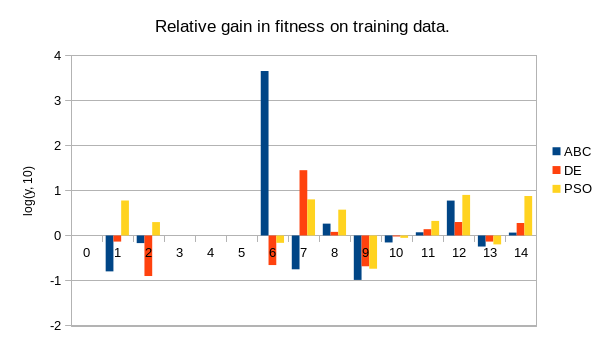
\includegraphics[width=0.8\linewidth]{figures/hybrid_phases10_mintrainfitness.png}
        \caption{Relative gain in best fitness of training data}
    \end{subfigure}%
    \begin{subfigure}{0.6\textwidth}
    \centering
        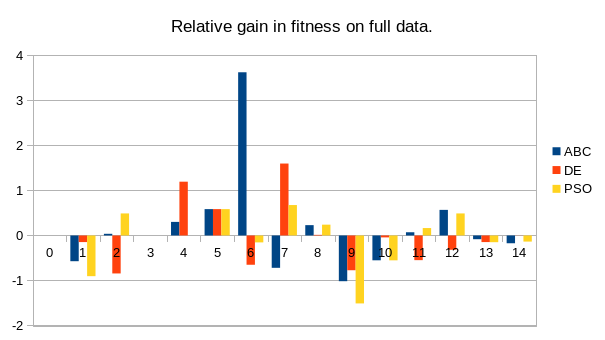
\includegraphics[width=0.8\linewidth]{figures/hybrid_phases10_minfullfitness.png}
        \caption{Relative gain in best fitness of full data}
    \end{subfigure}
        \begin{subfigure}{0.6\textwidth}
    \centering
        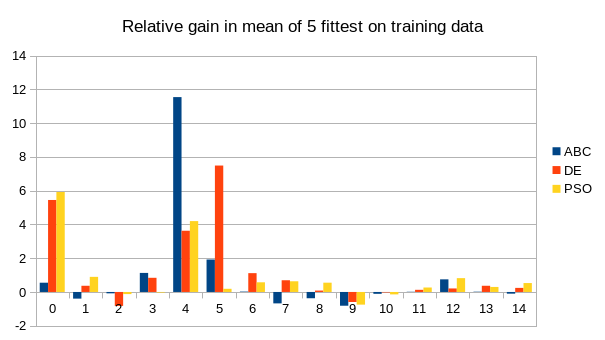
\includegraphics[width=0.8\linewidth]{figures/hybrid_phases10_meantrainfitness.png}
        \caption{Relative gain in mean fitness of training data}
    \end{subfigure}%
    \begin{subfigure}{0.6\textwidth}
    \centering
        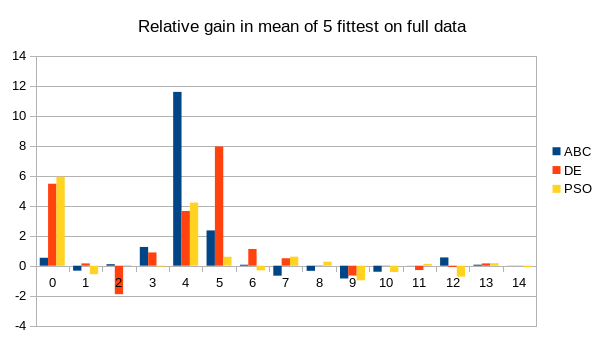
\includegraphics[width=0.8\linewidth]{figures/hybrid_phases10_meanfullfitness.png}
        \caption{Relative gain in mean fitness of full data}
    \end{subfigure}
    \caption{Relative gain of optimizer after 10 phases.}
    \label{fig:10phase}
    \end{figure}

% Table
\begin{landscape}
\begin{table}[]
\centering
\caption{Relative Gain in minimum fitness on training data after 10 phases.}
\label{table:10phasemintrain}
\begin{adjustbox}{width=1.7\textwidth}
\begin{tabular}{lllllllllllllllll}
     &           &           &           &           &           &           &           &           &           &           &           &           &           &           &           &  \\
 & 0         & 1         & 2         & 3         & 4         & 5         & 6         & 7         & 8         & 9         & 10        & 11        & 12        & 13        & 14        &  \\
ABC                 & 1.000e+00 & 1.591e-01 & 6.759e-01 & 1.000e+00 & 1.000e+00 & 1.000e+00 & 4.508e+03 & 1.771e-01 & 1.831e+00 & 1.029e-01 & 6.983e-01 & 1.176e+00 & 5.945e+00 & 5.674e-01 & 1.158e+00 &  \\
DE                  & 1.000e+00 & 7.304e-01 & 1.254e-01 & 1.000e+00 & 1.000e+00 & 1.000e+00 & 2.197e-01 & 2.816e+01 & 1.201e+00 & 2.068e-01 & 9.480e-01 & 1.377e+00 & 1.989e+00 & 7.304e-01 & 1.891e+00 &  \\
PSO                 & 1.000e+00 & 5.976e+00 & 1.980e+00 & 1.000e+00 & 1.000e+00 & 1.000e+00 & 6.857e-01 & 6.335e+00 & 3.739e+00 & 1.822e-01 & 8.852e-01 & 2.105e+00 & 7.945e+00 & 6.334e-01 & 7.526e+00 &  \\

\end{tabular}
\end{adjustbox}
\end{table}

\begin{table}[]
\centering
\caption{Gain in minimum fitness on full data after 10 phases.}
\label{table:10phaseminfull}
\begin{adjustbox}{width=1.7\textwidth}
\begin{tabular}{lllllllllllllllll}
         &           &           &           &           &           &           &           &           &           &           &           &           &           &           &           &  \\
         & 0         & 1         & 2         & 3         & 4         & 5         & 6         & 7         & 8         & 9         & 10        & 11        & 12        & 13        & 14        &  \\
ABC                 & 1.000e+00 & 2.679e-01 & 1.087e+00 & 1.000e+00 & 2.000e+00 & 3.846e+00 & 4.224e+03 & 1.908e-01 & 1.694e+00 & 9.627e-02 & 2.807e-01 & 1.178e+00 & 3.699e+00 & 8.255e-01 & 6.709e-01 &  \\
DE                  & 1.000e+00 & 7.126e-01 & 1.432e-01 & 1.000e+00 & 1.565e+01 & 3.846e+00 & 2.232e-01 & 3.965e+01 & 1.031e+00 & 1.687e-01 & 9.052e-01 & 2.827e-01 & 4.813e-01 & 7.126e-01 & 1.005e+00 &  \\
PSO                 & 1.000e+00 & 1.246e-01 & 3.083e+00 & 1.000e+00 & 1.000e+00 & 3.846e+00 & 7.019e-01 & 4.738e+00 & 1.736e+00 & 3.091e-02 & 2.797e-01 & 1.459e+00 & 3.081e+00 & 7.083e-01 & 7.305e-01 &  \\

\end{tabular}
\end{adjustbox}
\end{table}

\begin{table}[]
\centering
\caption{Relative gain in mean fitness of 5 fittest expressions on training data after 10 phases.}
\label{table:10phasemeantrain}
\begin{adjustbox}{width=1.7\textwidth}
\begin{tabular}{lllllllllllllllll}
 &           &           &           &           &           &           &           &           &           &           &           &           &           &           &           &  \\
 & 0         & 1         & 2         & 3         & 4         & 5         & 6         & 7         & 8         & 9         & 10        & 11        & 12        & 13        & 14        &  \\
ABC                 & 3.530e+00 & 4.032e-01 & 8.301e-01 & 1.346e+01 & 3.503e+11 & 8.400e+01 & 1.061e+00 & 2.112e-01 & 4.251e-01 & 1.531e-01 & 7.788e-01 & 1.034e+00 & 5.595e+00 & 1.041e+00 & 7.932e-01 &  \\
DE                  & 2.813e+05 & 2.333e+00 & 1.492e-01 & 6.914e+00 & 4.242e+03 & 3.098e+07 & 1.305e+01 & 4.957e+00 & 1.210e+00 & 2.547e-01 & 9.384e-01 & 1.339e+00 & 1.614e+00 & 2.333e+00 & 1.742e+00 &  \\
PSO                 & 8.346e+05 & 7.871e+00 & 7.495e-01 & 9.256e-01 & 1.573e+04 & 1.539e+00 & 3.743e+00 & 4.297e+00 & 3.560e+00 & 1.781e-01 & 7.192e-01 & 1.838e+00 & 6.612e+00 & 1.991e+00 & 3.372e+00 &  \\
\end{tabular}
\end{adjustbox}
\end{table}


\begin{table}[]
\centering
\caption{Relative gain in mean fitness of 5 fittest expressions on full data after 10 phases.}
\label{table:10phasemeanfull}
\begin{adjustbox}{width=1.7\textwidth}
\begin{tabular}{lllllllllllllllll}
     &           &           &           &           &           &           &           &           &           &           &           &           &           &           &           &  \\
     & 0         & 1         & 2         & 3         & 4         & 5         & 6         & 7         & 8         & 9         & 10        & 11        & 12        & 13        & 14        &  \\
ABC                 & 3.389e+00 & 4.674e-01 & 1.263e+00 & 1.779e+01 & 3.846e+11 & 2.257e+02 & 1.163e+00 & 2.171e-01 & 4.563e-01 & 1.408e-01 & 3.961e-01 & 1.020e+00 & 3.568e+00 & 1.170e+00 & 1.027e+00 &  \\
DE                  & 2.901e+05 & 1.426e+00 & 1.270e-02 & 7.677e+00 & 4.445e+03 & 8.874e+07 & 1.310e+01 & 3.143e+00 & 1.057e+00 & 2.200e-01 & 9.597e-01 & 5.134e-01 & 8.172e-01 & 1.426e+00 & 1.039e+00 &  \\
PSO                 & 8.487e+05 & 2.720e-01 & 1.113e+00 & 8.726e-01 & 1.601e+04 & 3.942e+00 & 4.913e-01 & 4.000e+00 & 1.855e+00 & 1.070e-01 & 3.816e-01 & 1.327e+00 & 1.873e-01 & 1.466e+00 & 8.262e-01 & 
\end{tabular}
\end{adjustbox}
\end{table}
\end{landscape}

\subsubsection{Cost}
The cost in terms of evaluations is linear in the number of phases. For each phase, 4 expressions are optimized with O(nk) complexity. In our configuration n=50, k=50. The SR algorithm itself requires O(mg) evaluations per phase, where m is the population (20) and g the generations per phase (20). The question whether or not the cost of the optimizer is worth the gain in fitness is in the end one for the practitioner to answer. There is no guarantee that improvement will take place, but from the results on the above hard problems we can still expect significant improvements up to several orders of magnitude.

\subsection{Distributed}
We now apply our tool to the testproblems in a distributed setup.

\subsubsection{Experiment setup}
\begin{itemize}
\item population : 20
\item minimum depth : 4
\item maximum depth : 8
\item phases : 20
\item generations per phase : 20
\item datapoints : 20
\item range : [1,5]
\item features : 5
\item archivesize : 20
\item expressions to archive per phase : 4
\item optimization strategy : none
\item communication size m : 2, 4
\item topology : Tree, Random, Grid
\item spreadpolicy : distribute
\item processes n : 25
\end{itemize}
\paragraph{Discussion}
From section \ref{subsec:commstrategies}
we know that simply using m for all topologies will lead to unintended communication patterns. We test Tree and Random with m = 2, and Grid with m = 4. This results in the following number of messages per link :
\begin{itemize}
\item Grid : 1
\item Tree : 1
\item Random : 2
\end{itemize}
The total number of messages sent per phase is then :
\begin{itemize}
\item Grid : 4 * n = 200
\item Tree : 1 * n = 25
\item Random : 2 * n = 50
\end{itemize}
The value of m = 2 for Tree and m = 4 for Grid follows from our discussion in \ref{subsec:commstrategies}. The Random topology in this configuration has a single outgoing link per process, resulting in 2 messages per link. This configuration forms a balance between the different strategies.

\subsubsection{Measures}
When the experiment ends the best 20 expressions from all processes are collected and scored. We measure in best fitness on the training data, and best fitness on the validated data. As we have seen in % todo ref kfold 
there is a subtle difference here compared to the sequential approach. While each process has a subset of the training and validation data, in the end we score against the full dataset.
Finally we record the mean fitness values of the best 5 expressions, both on the training and validation data. These are the same measures as used by the optimizer experiment. The mean is restricted to the upper quarter of the population specifically to measure how the best expressions are distributed. This measure records the convergence more accurately as the fittest expressions drive the convergence rate. 
\paragraph{Calculation}
The fitness values fluctuate strongly between the test problems and even between topologies. We apply a negative logarithmic scale :
\[
f_t = -\log_{10}(f)
\]
where f is either the best fitness value or the mean. Then we scale the results relative to the values obtained for the tree topology in order to measure relative gain or loss in orders of magnitude.
\[
v_{t} = \frac{f_{t}}{f_{tree}}
\]
\subsection{Conclusion}
\subsubsection{Operator cooling schedule}
\subsubsection{Constant folding}
\subsubsection{Optimizers}
The experiments with the optimizers highlight several issues. There are a wide number of strategies and parameters that influence the effect of the optimizer. We also see that optimizers can hinder the algorithm in its convergence. This is not a general conclusion, but dependent in part on our design choices and the trade-offs made. If we only optimize the final outcome of the algorithm it is obvious that no fitness regression is possible. Only when we apply optimization in the archiving stage are there subtle effects at play that allow for such edge cases. The cost of applying the optimizers is significant. In our implementation the cost is known beforehand, but the gain is not. This holds true in general for this GP SR algorithm. While we can empirically investigate the convergence of a number of problems, there is no known limit to this process. 
In general, when the optimizers are used the improvements made are far greater than the loss in edge cases. We have tested 3 distinct algorithms as optimizers in order to test which is best. Unfortunately no such algorithm exists. The NFL theorem \cite{NFL} suggests as much. What we can see is that ABC and DE offer, for our problem set, the best results. Best in this context means the overall highest gain with the lowest losses at an equal cost to the other algorithms. The hardness of the SR problem indicates that, unfortunately, there are an infinite number of problem statements that will have different convergence characteristics. While hybridization of the GP algorithm with other algorithms is a viable strategy, it also substantially increases the number of parameters. 